\documentclass[12pt]{article}
\usepackage[margin=1in]{geometry}     
\usepackage{graphicx}
\usepackage{epstopdf}
\setlength\parindent{0pt}
\usepackage{natbib}
\usepackage{booktabs}
\bibliographystyle{plainnat}
\usepackage{soul}
\usepackage{subcaption}
\usepackage{booktabs}
\usepackage{array}
\usepackage{threeparttable}
\usepackage{rotating}
\usepackage{pdflscape}
\usepackage[fleqn]{amsmath}

\usepackage[format=plain,
labelfont=it,
textfont=it]{caption}

%opening
\title{Relative Impacts of pCO$_{2}$ Constituents}
\author{Riley X. Brady}
\date{\today}


\begin{document}

\maketitle
\begin{abstract}
\noindent We found through the first phase of the project that raw pCO$_{2}$ values are the dominant predictor of CO$_{2}$ flux variability in EBUS. Interestingly, upon partitioning pCO$_{2}$ into temperature-dependent and non-temperature-dependent, we found that certain systems aligned with each class. The CalCS, for instance, had very strong correlations with temperature-dependent pCO$_{2}$ (as well as raw SSTs, of course). However, the other three systems were very well-predicted by non-temperature-dependent factors. But what exactly are the major factors? Here, we use a linear Taylor Series decomposition to understand what major BGC factors change during a natural climate event (e.g. El Ni\~no).
\end{abstract}

\newpage
\section{pCO$_{2}$ Correlations}
Per \citet{Takahashi2002} and \citet{Fay2013}, we can use empirical equations to create a temperature-dependent pCO$_{2}$ time series (that holds pCO$_{2}$ constant and allows SST to vary) and a non-temperature-dependent pCO$_{2}$ that fixes SST and allows DIC, Alk, and salinity to play a role:
$$
	pCO_{2}-T = \textrm{mean}~pCO_{2} \times \exp(0.0423 \times (SST_{obs} - SST_{mean}))
$$
$$
	pCO_{2}-nonT = \textrm{obs}~pCO_{2} \times \exp(0.0423 \times (SST_{mean} - SST_{obs}))
$$

We complete this on a simulation-by-simulation basis, using the total time series (forced signal + residuals). After partitioning into pCO$_{2}$-T and pCO$_{2}$-non-T, we detrend each component via a 4th order polynomial fit. This removes the clear anthropogenic trend in the non-T component and allows us to correlate the stationary variability to CO$_{2}$ flux anomalies. Figure~\ref{fig:pco2-decomposition} displays the partitioning of a pCO$_{2}$ time series in the CalCS into its temperature and non-temperature dependent components. The bottom two subplots are detrended after this step and then correlated to CO$_{2}$ flux residuals. \\

We find that the CalCS is most positively correlated to pCO$_{2}$-T (Figure~\ref{fig:pCO2-T-histograms}), likely suggesting that this is a solubility-dependent system. On the other hand, the HumCS is very negatively correlated to pCO$_{2}$-T, such that there is anomalous CO$_{2}$ uptake during a warm event. Since this doesn't make sense from the argument of solubility, this likely suggests that the warm SST anomalies coincide with a circulation suppression. We might consider the HumCS a circulation-dependent system. Figure~\ref{fig:pCO2-nonT-histograms} displays the results of correlations with the non-temperature-dependent pCO$_{2}$ time series. We find here that the CalCS hovers around the zero-line for correlations. On the other hand, the remaining three systems are very well explained by this variable. This could suggest that the other systems are driven by other terms that pCO$_{2}$ depends on.

In the next section, we will use a linear Taylor Expansion to further nail down the relative effects of SST, SALT, DIC, and ALK on pCO$_{2}$ variability, which is the dominant driver of CO$_{2}$ flux variability.


\clearpage
\begin{figure*}[!h]
	\centering
	\begin{subfigure}[b]{\textwidth}
		\centering
		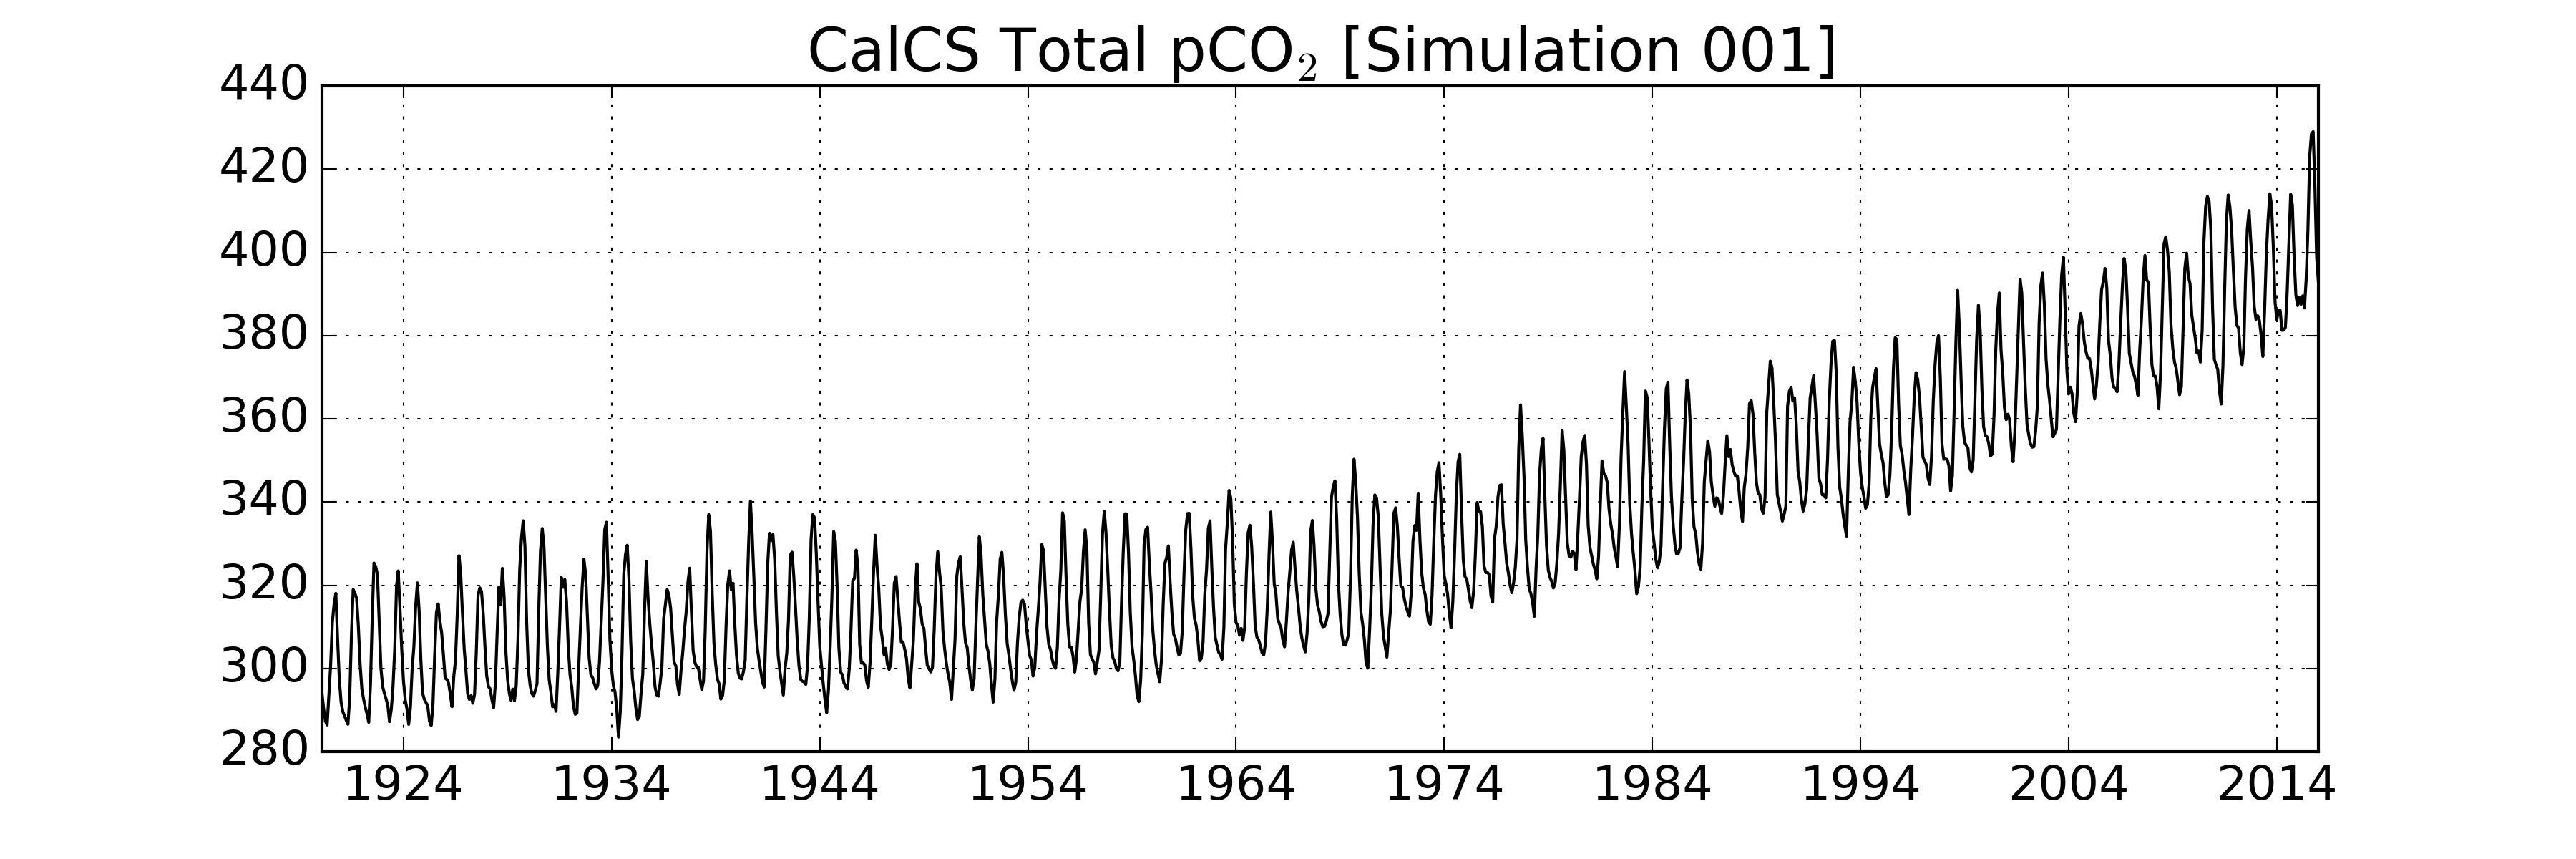
\includegraphics[width=\linewidth]{../../figs/calcs/timeseries/calcs-total-pco2-001.png}
	\end{subfigure} \\
	\begin{subfigure}[b]{\textwidth}
		\centering
		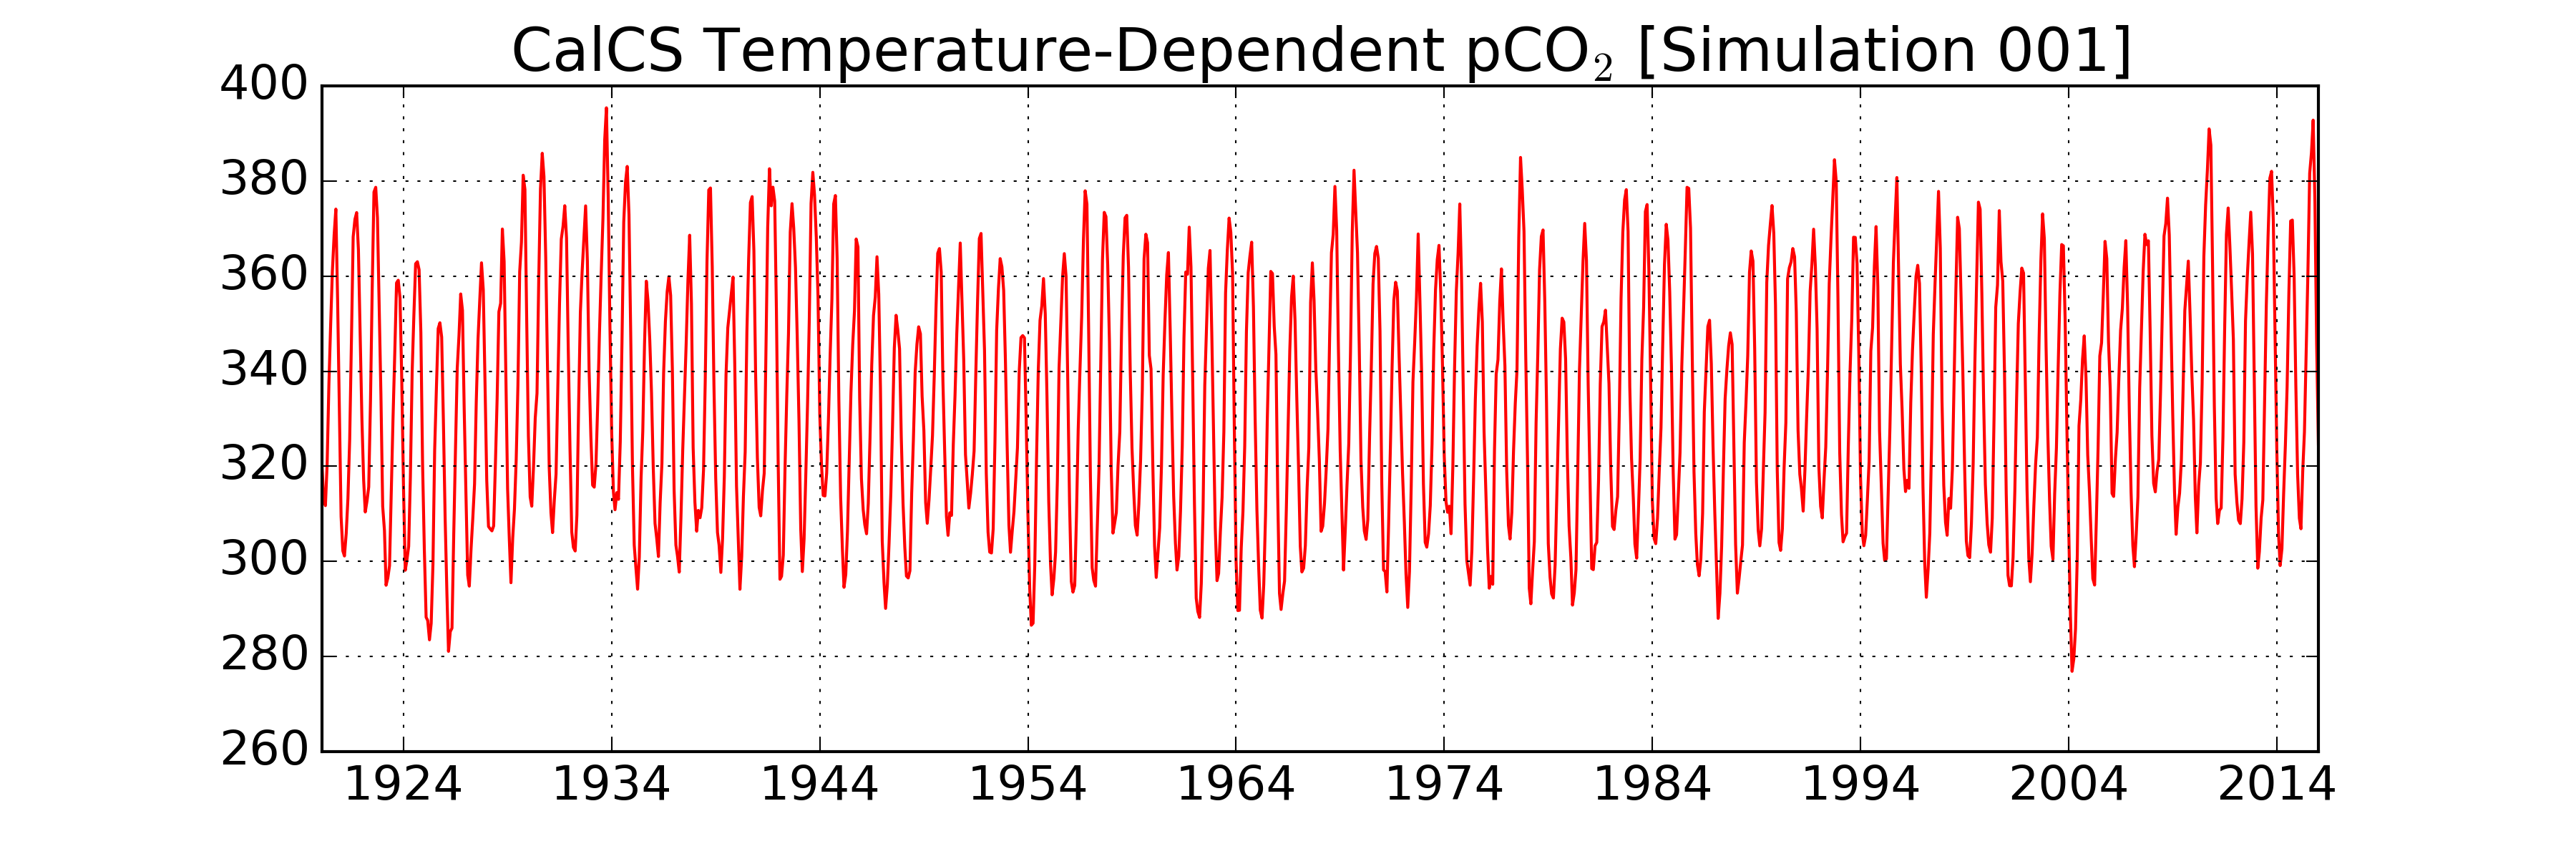
\includegraphics[width=\linewidth]{../../figs/calcs/timeseries/calcs-pCO2_T-pco2-001.png}
	\end{subfigure} \\
	\begin{subfigure}[b]{\textwidth}
		\centering
		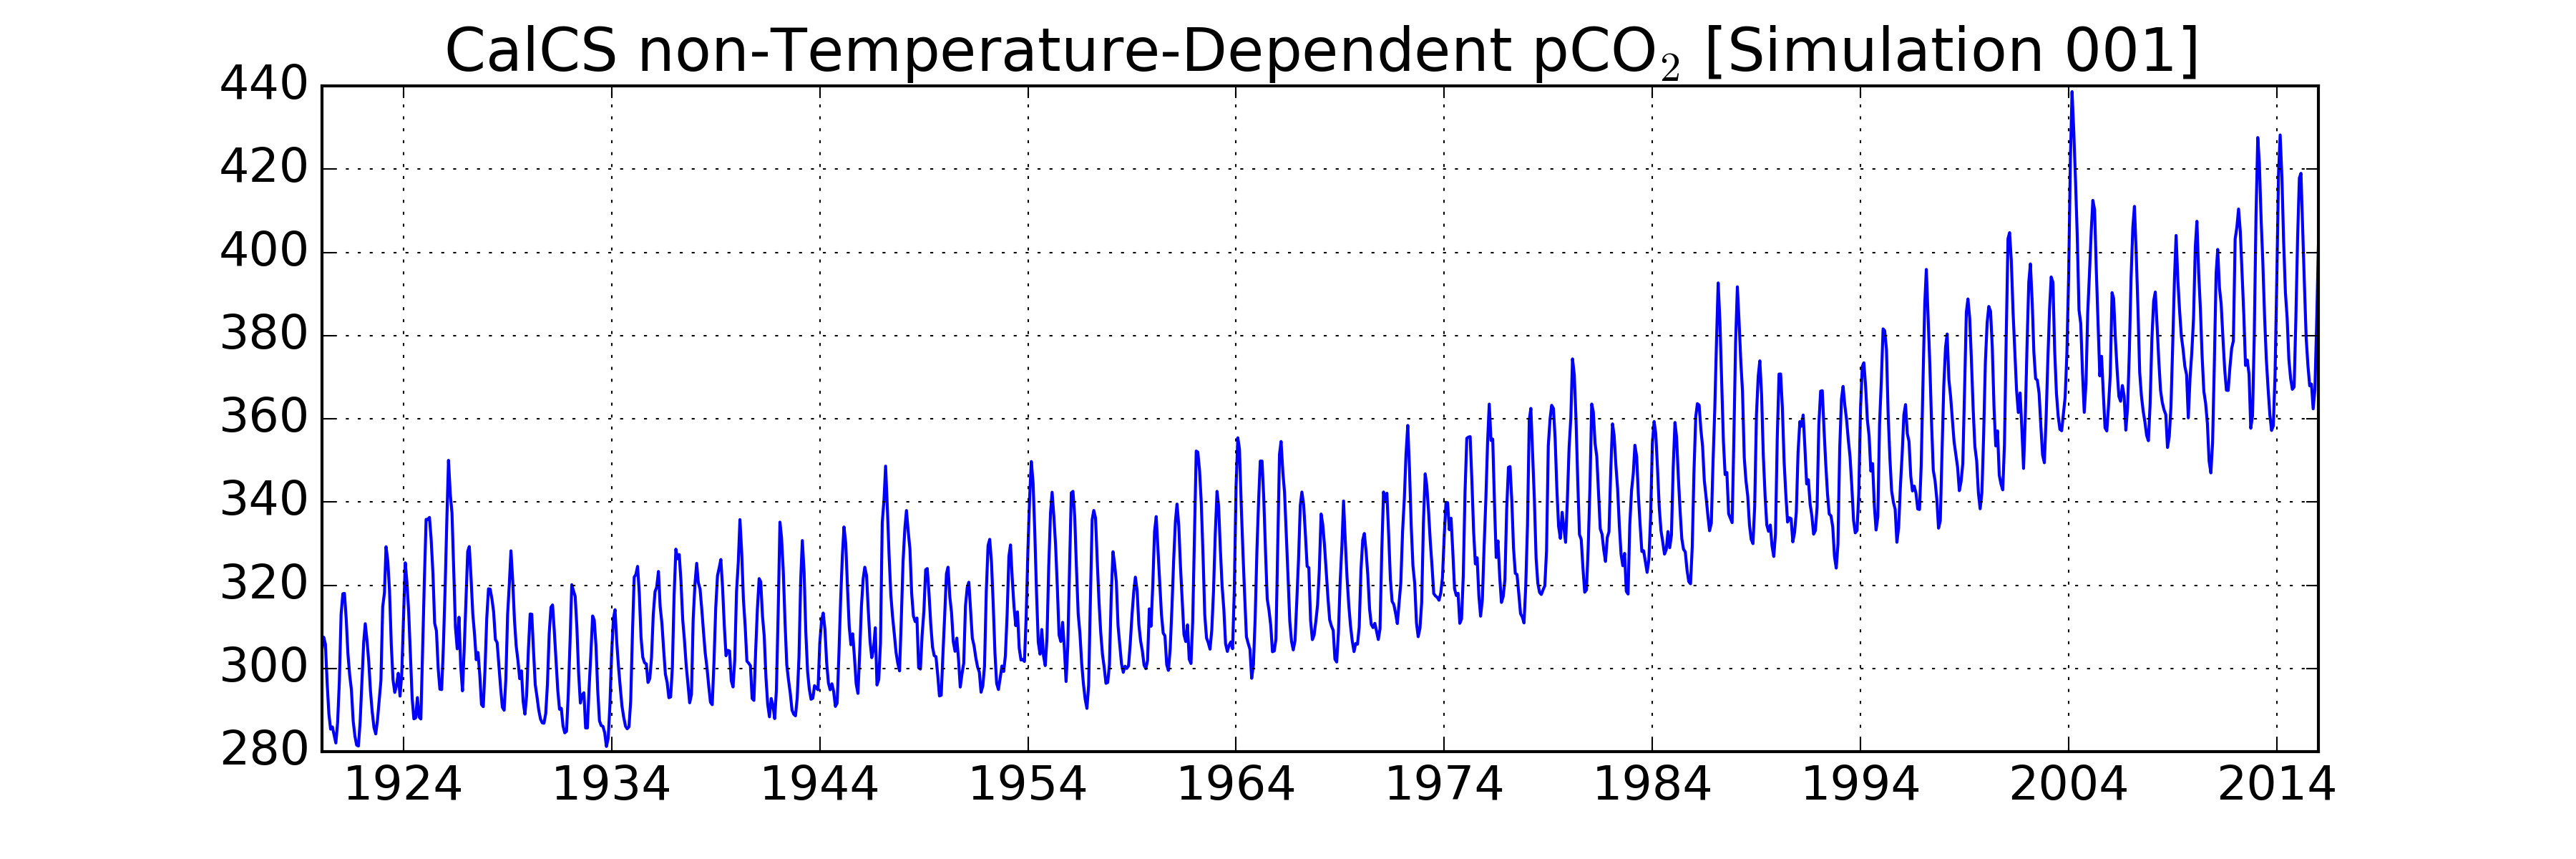
\includegraphics[width=\linewidth]{../../figs/calcs/timeseries/calcs-pCO2_nonT-pco2-001.png}
	\end{subfigure} 
	\caption{Example of partitioning a total pCO$_{2}$ time series into its temperature and non-temperature dependent pieces, via methodology from \citet{Takahashi2002}}
	\label{fig:pco2-decomposition}
\end{figure*}

\clearpage
\begin{figure}[!h]
	\centering
	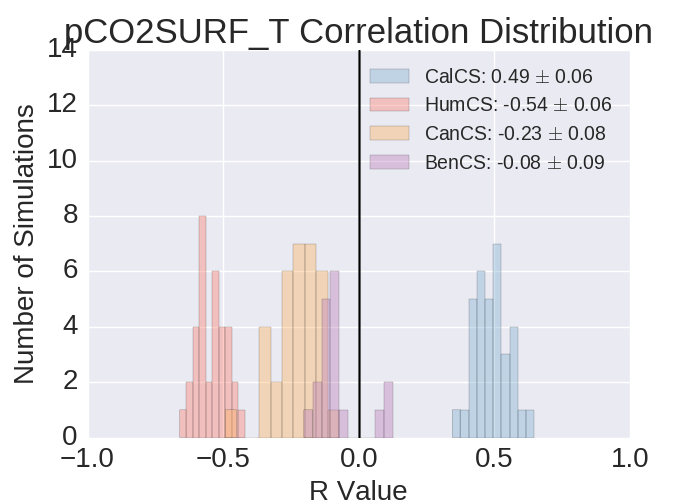
\includegraphics[width=25pc]{../../figs/all-systems/histograms/pCO2SURF_T-correlation-distributions.png}
	\caption{Distributions of correlations between the temperature-dependent pCO$_{2}$ anomalies and FGCO2 anomalies in all four EBUS.}
	\label{fig:pCO2-T-histograms}
\end{figure}
\begin{figure}[!h]
	\centering
	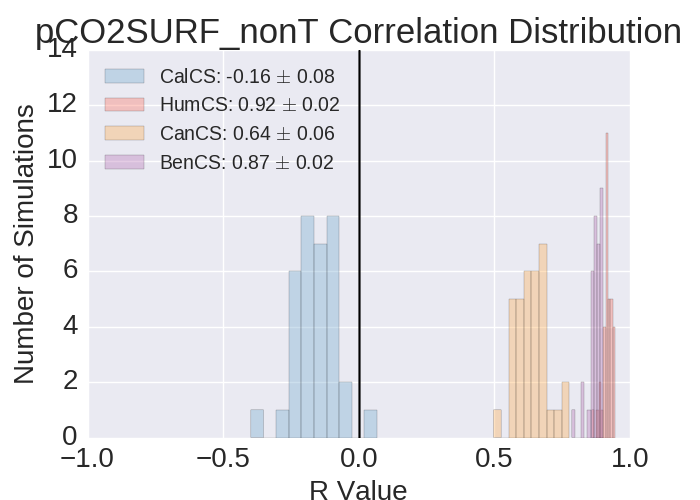
\includegraphics[width=25pc]{../../figs/all-systems/histograms/pCO2SURF_nonT-correlation-distributions.png}
	\caption{Distributions of correlations between the non-temperature-dependent pCO$_{2}$ anomalies and FGCO2 anomalies in all four EBUS.}
	\label{fig:pCO2-nonT-histograms}
\end{figure}

\newpage
\section{Linear Taylor Expansion}
pCO$_{2}$ concentrations are determined by dissolved inorganic carbon (DIC), alkalinity (ALK), sea surface temperature (SST), and sea surface salinity (SALT). Given a pCO$_{2}$ perturbation, \it e.g.\rm, from an ENSO event, we can look at which of the four aforementioned terms played the largest role. The expansion is as follows (\citet{Lovenduski2007} and \citet{Lovenduski2015}):
\begin{equation}
	\Delta pCO_{2} = \frac{\partial pCO_{2}}{\partial DIC}\Delta DIC + \frac{\partial pCO_{2}}{\partial ALK}\Delta ALK + \frac{\partial pCO_{2}}{\partial SST}\Delta SST + \frac{\partial pCO_{2}}{\partial SALT}\Delta SALT
\end{equation}

We find the partial derivative terms (pCO$_{2}$ sensitives) by using empirical equations from \citet{Takahashi1993} and CESM-LE ensemble mean output for each region. First, I will outline the equations that lead to discovering the sensitivities, and then follow with a table of those fixed sensitivities for each term and EBUS over the 1920-2015 period. To clarify, we find non-derivative values (such as pCO$_{2}$ in Equation 2) by taking the CESM-LE ensemble mean over the given EBUS from 1920-2015, and they remain constant for these analyses.

\begin{equation}
	\frac{\partial pCO_{2}}{\partial SST} \approx 0.0423^{o}C^{-1}\cdot pCO_{2}
\end{equation}

\begin{equation}
	\frac{\partial pCO_{2}}{\partial SALT} \approx \frac{pCO_{2}}{SALT}
\end{equation}

\begin{equation}
	\frac{\partial pCO_{2}}{\partial DIC} = \frac{pCO_{2}}{DIC}\gamma_{DIC}
\end{equation}
where $ \gamma_{DIC} = \frac{3\cdot ALK\cdot DIC - 2DIC^{2}}{(2DIC - ALK)(ALK - DIC)} $

\begin{equation}
	\frac{\partial pCO_{2}}{\partial ALK} = \frac{pCO_{2}}{ALK}\gamma_{ALK}
\end{equation}
where $ \gamma_{ALK} = -\frac{ALK^{2}}{(2DIC - ALK)(ALK-DIC)} $

\vspace{0.5cm}
The delta terms from Equation 1 (\it e.g.\rm, $\Delta DIC$) are computed by regressing the variable of interest onto the climate index of choice. For instance, if we were investigating ENSO, we would use Nino3.4 as the predictor (x), and DIC as the dependent variable (y). The regression slope would be our delta term, and thus the entire equation would be relative to 1$\sigma$ or 1 degree C of warming related to ENSO.

\clearpage
\begin{table}
	\centering
	\caption{pCO$_{2}$ sensitivities and buffer factors for DIC and ALK for each EBUS. These values are assumed constant over the historical period for each simulation and are used in the Taylor expansion (Equation 1).}	
	\begin{tabular}{c c c c c}
		\toprule
		Term & CalCS  &  HumCS &  CanCS & BenCS \\
		\midrule
		\multicolumn{5}{c}{Sensitivities}  \\[0.1cm]
		$\frac{\partial pCO_{2}}{\partial SST}$ &  14.03 & 17.11  & 14.74 & 15.52 \\ [0.5cm]
		$\frac{\partial pCO_{2}}{\partial SALT}$ &  10.23 & 11.62 & 9.69 & 10.28 \\ [0.5cm]
		$\frac{\partial pCO_{2}}{\partial DIC}$ &  2.28 & 2.37 & 1.85 & 2.07 \\ [0.5cm]
		$\frac{\partial pCO_{2}}{\partial ALK}$ &  -1.90 & -1.91 & -1.44 & -1.66 \\ 
		\midrule
		\multicolumn{5}{c}{Buffer Factors}  \\ [0.1cm]
		$\gamma_{DIC}$ & 13.42 & 11.95 & 10.84 & 11.72 \\ [0.5cm]
		$\gamma_{ALK}$ & -12.42 & -10.95 & -9.84 & -10.72 \\ 
		\bottomrule
	\end{tabular}
	\label{tab:pCO2-sensitivities}
\end{table}

\clearpage
\begin{figure}[!h]
	\centering
	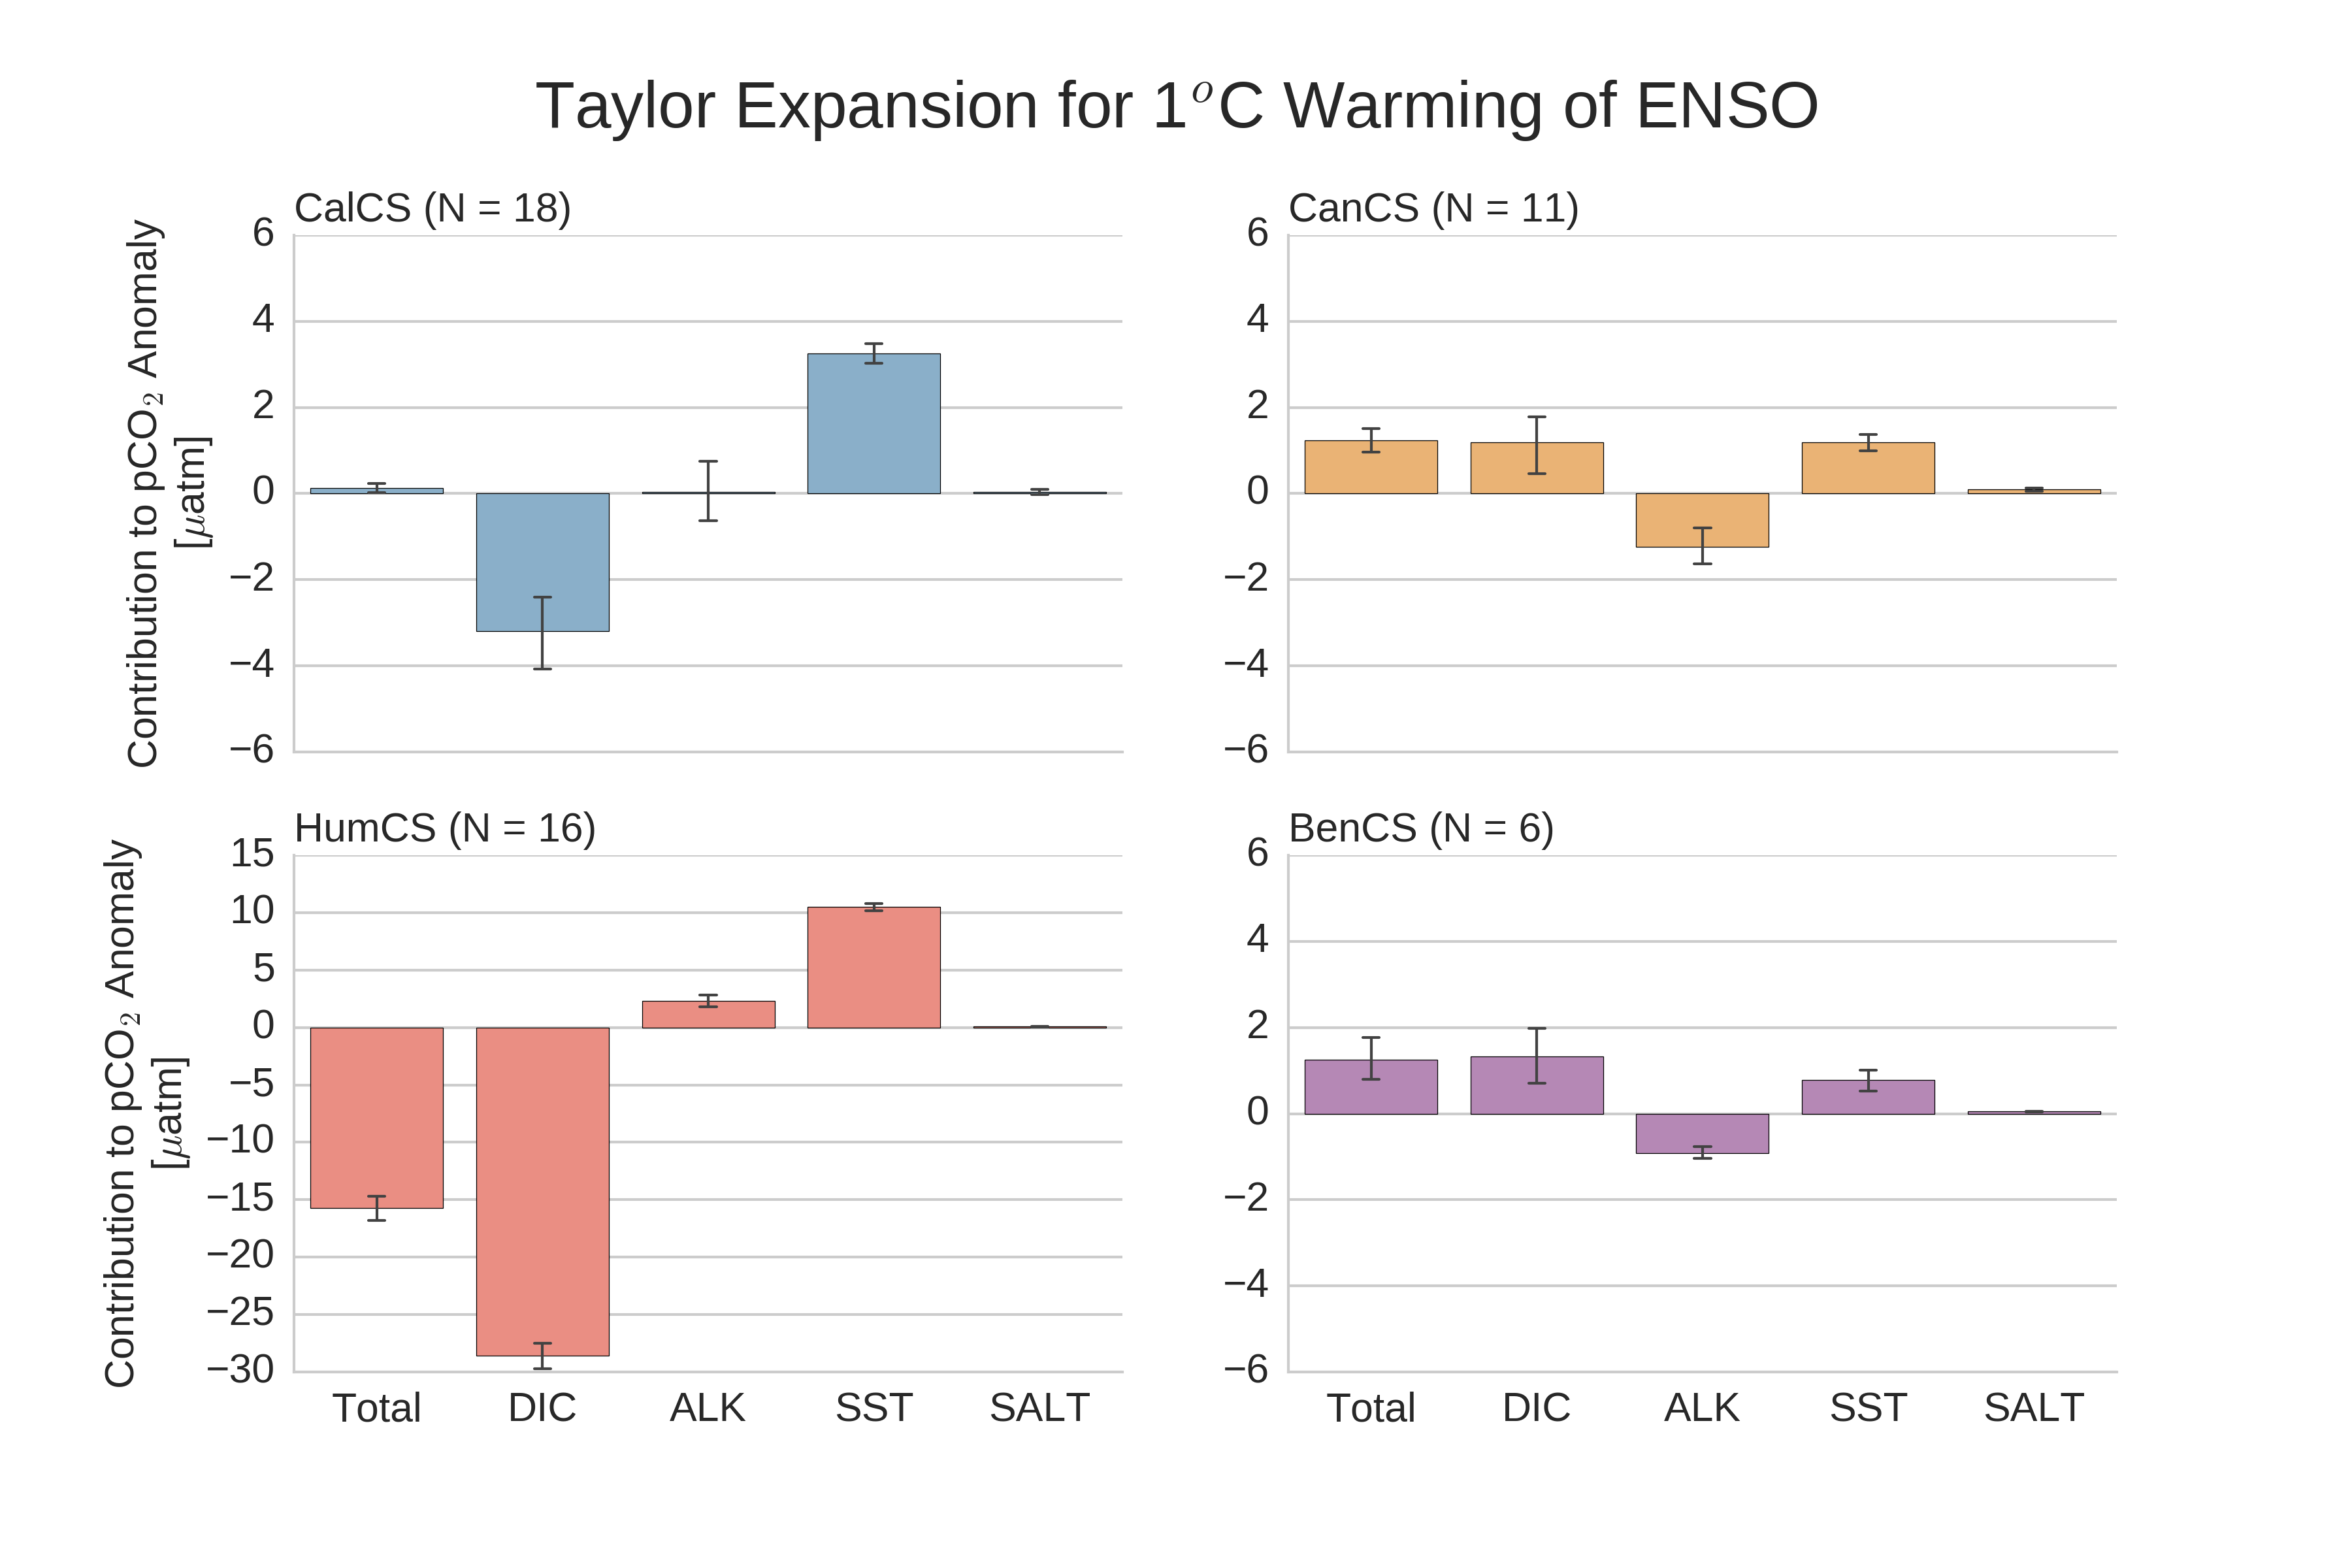
\includegraphics[width=\linewidth]{../../figs/all-systems/taylor_expansions/taylor-expansion-ENSO-pCO2-PVALUEREMOVED-smoothedClimate.png}
	\caption{Linear Taylor Expansion of the relative contributions toward pCO$_{2}$ anomalies in a 1 degree C El Ni\~no event. Only simulations with $p$ $<$ 0.05 for pCO2, SALT, SST, ALK, and DIC were included.}
	\label{fig:taylor-enso}
\end{figure}
\begin{table}[!h]
	\centering
\begin{tabular}{c | c c c c }
	& CalCS & HumCS & CanCS & BenCS \\
	\midrule
	Model Regression & 0.67 & -13.16 & 0.98 & 1.27 \\
	Taylor Summation & 0.12 & -15.72 & 1.24 & 1.25 \\
\end{tabular}
	\caption{Comparison between regressing pCO$_{2}$ anomalies onto ENSO and the summation of each term of the linear taylor approximation for each system}
	\label{tab:taylor-enso}
\end{table}

\clearpage
\begin{figure}[!h]
	\centering
	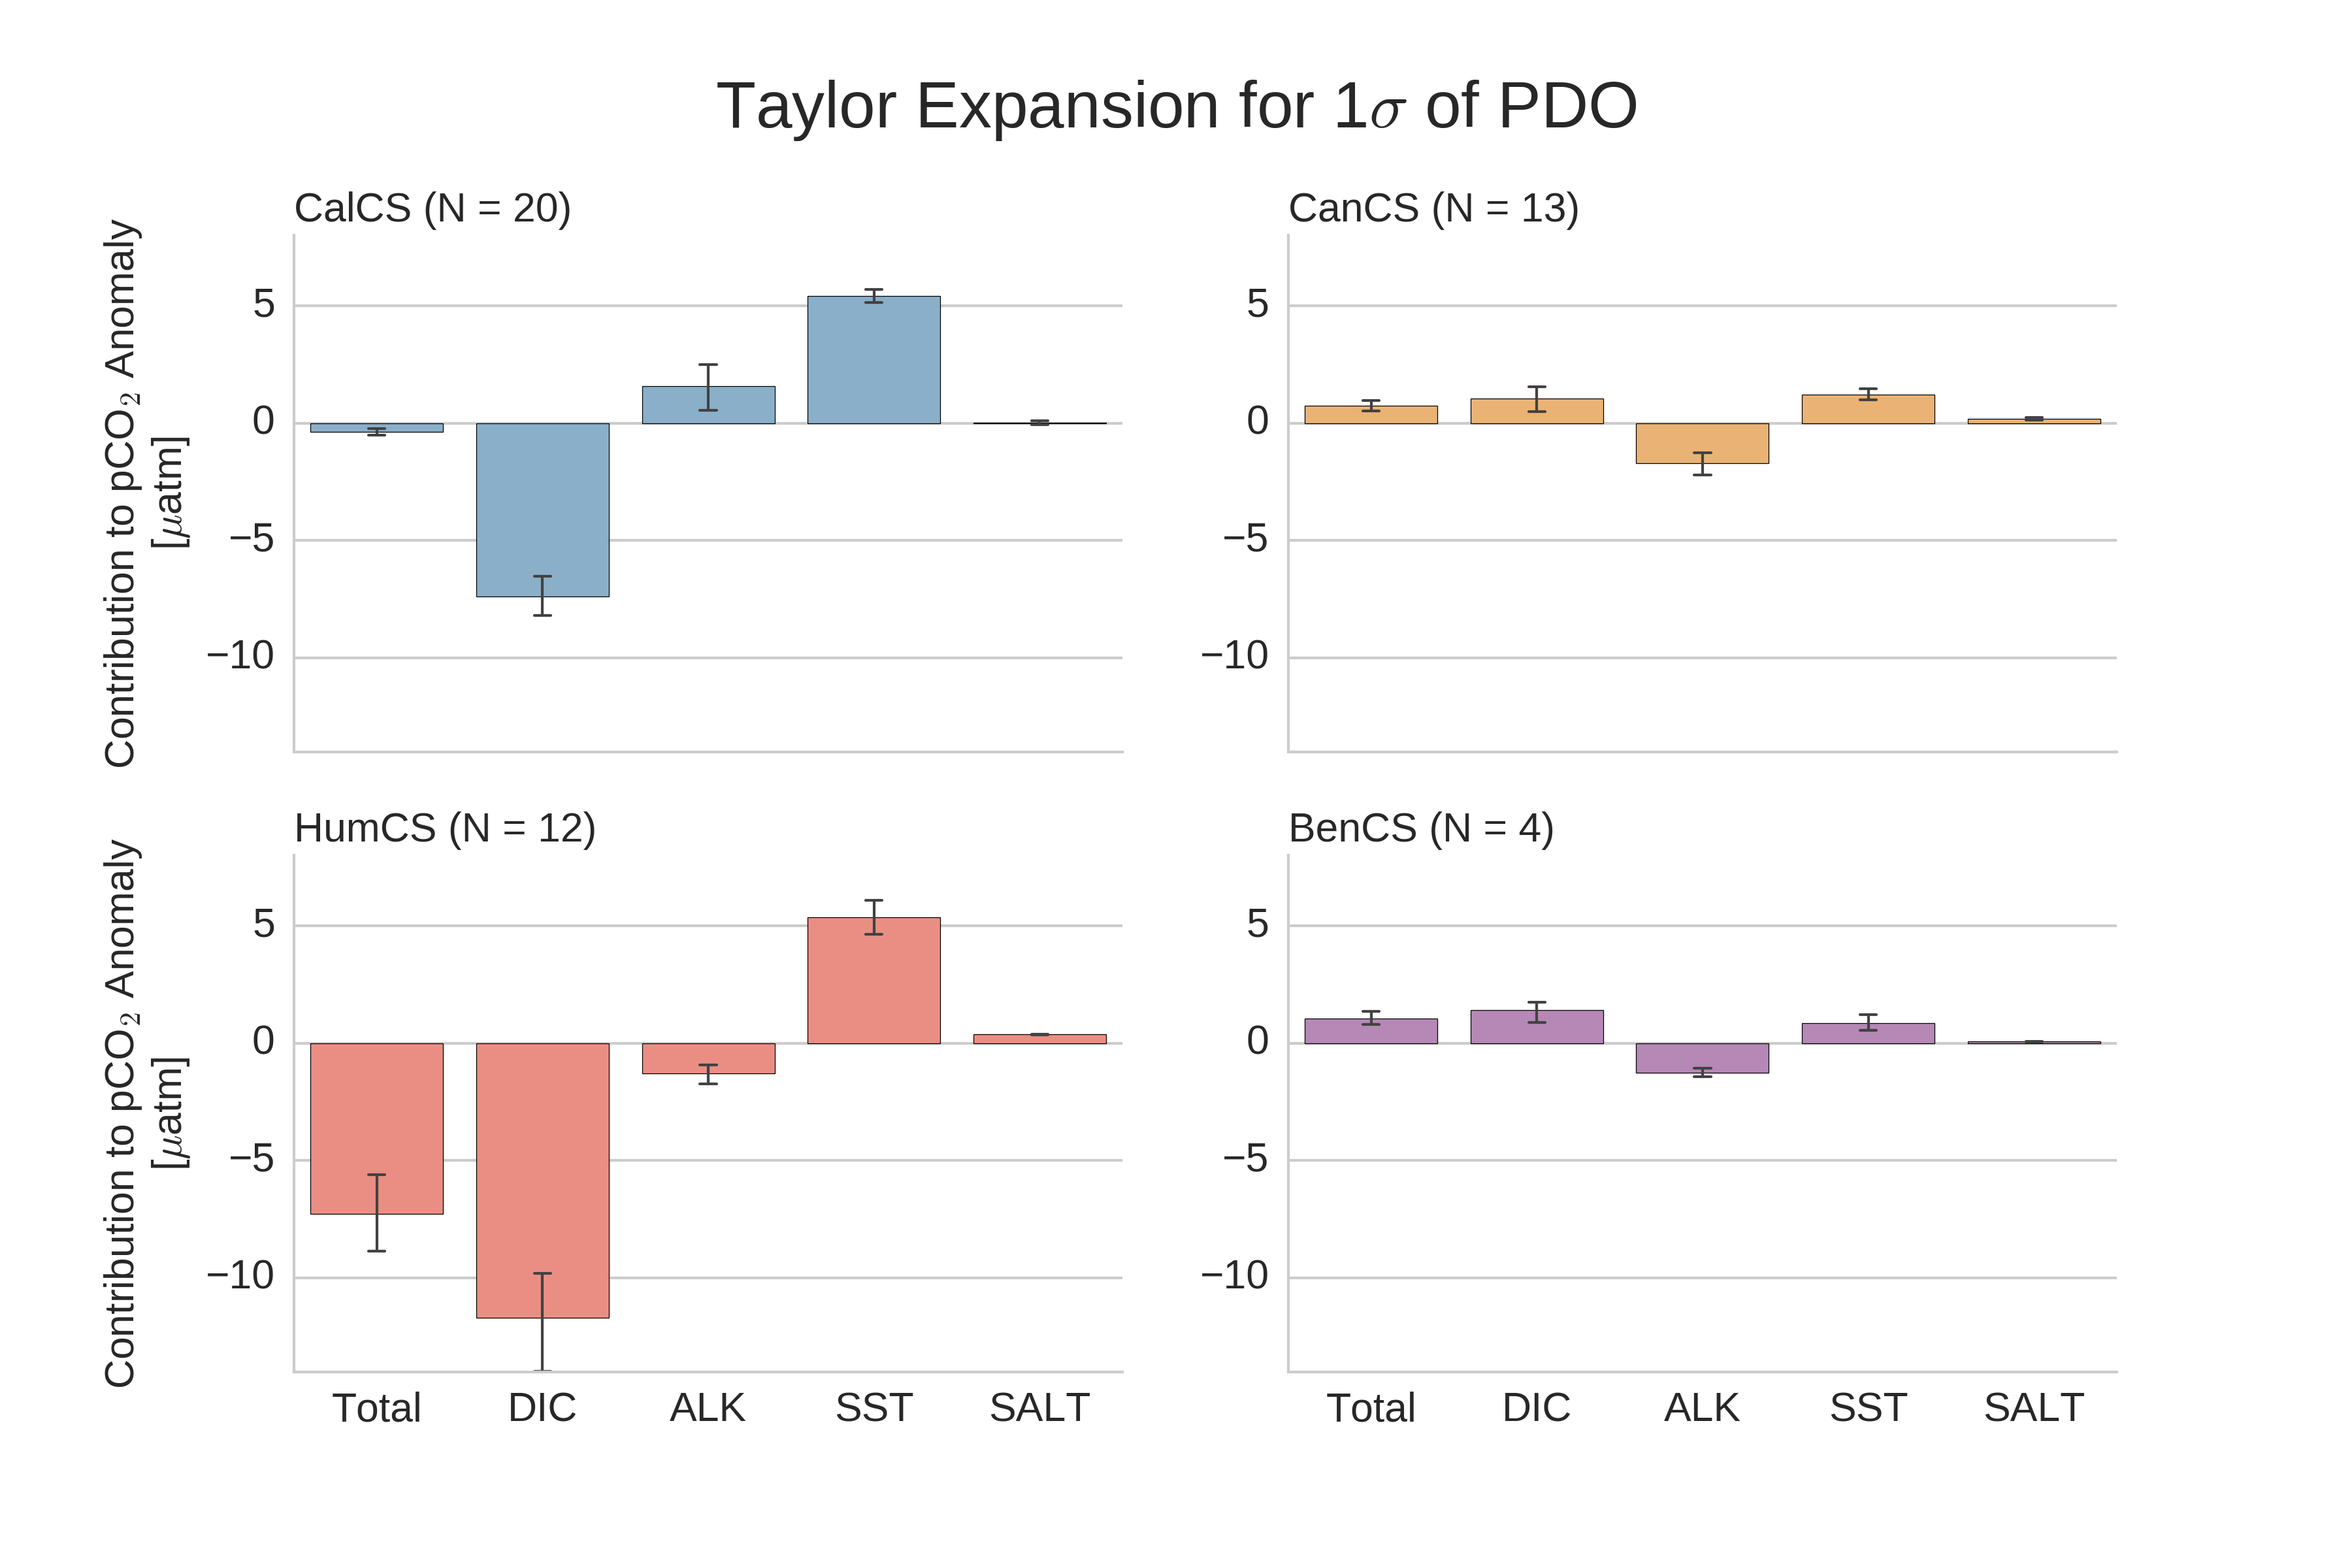
\includegraphics[width=\linewidth]{../../figs/all-systems/taylor_expansions/taylor-expansion-PDO-pCO2-PVALUEREMOVED-smoothedClimate.png}
	\caption{Linear Taylor Expansion of the relative contributions toward pCO$_{2}$ anomalies in a 1 $\sigma$ PDO event. Only simulations with $p$ $<$ 0.05 for pCO2, SALT, SST, ALK, and DIC were included.}
	\label{fig:taylor-pdo}
\end{figure}
\begin{table}[!h]
	\centering
	\begin{tabular}{c | c c c c }
		& CalCS & HumCS & CanCS & BenCS \\
		\midrule
		Model Regression & 0.65 & -5.37 & 0.66 & 1.10 \\
		Taylor Summation & -0.37 & -7.27 & 0.73 & 1.05 \\
	\end{tabular}
	\caption{Comparison between regressing pCO$_{2}$ anomalies onto PDO and the summation of each term of the linear taylor approximation for each system}
	\label{tab:taylor-pdo}
\end{table}

\clearpage
\begin{figure}[!h]
	\centering
	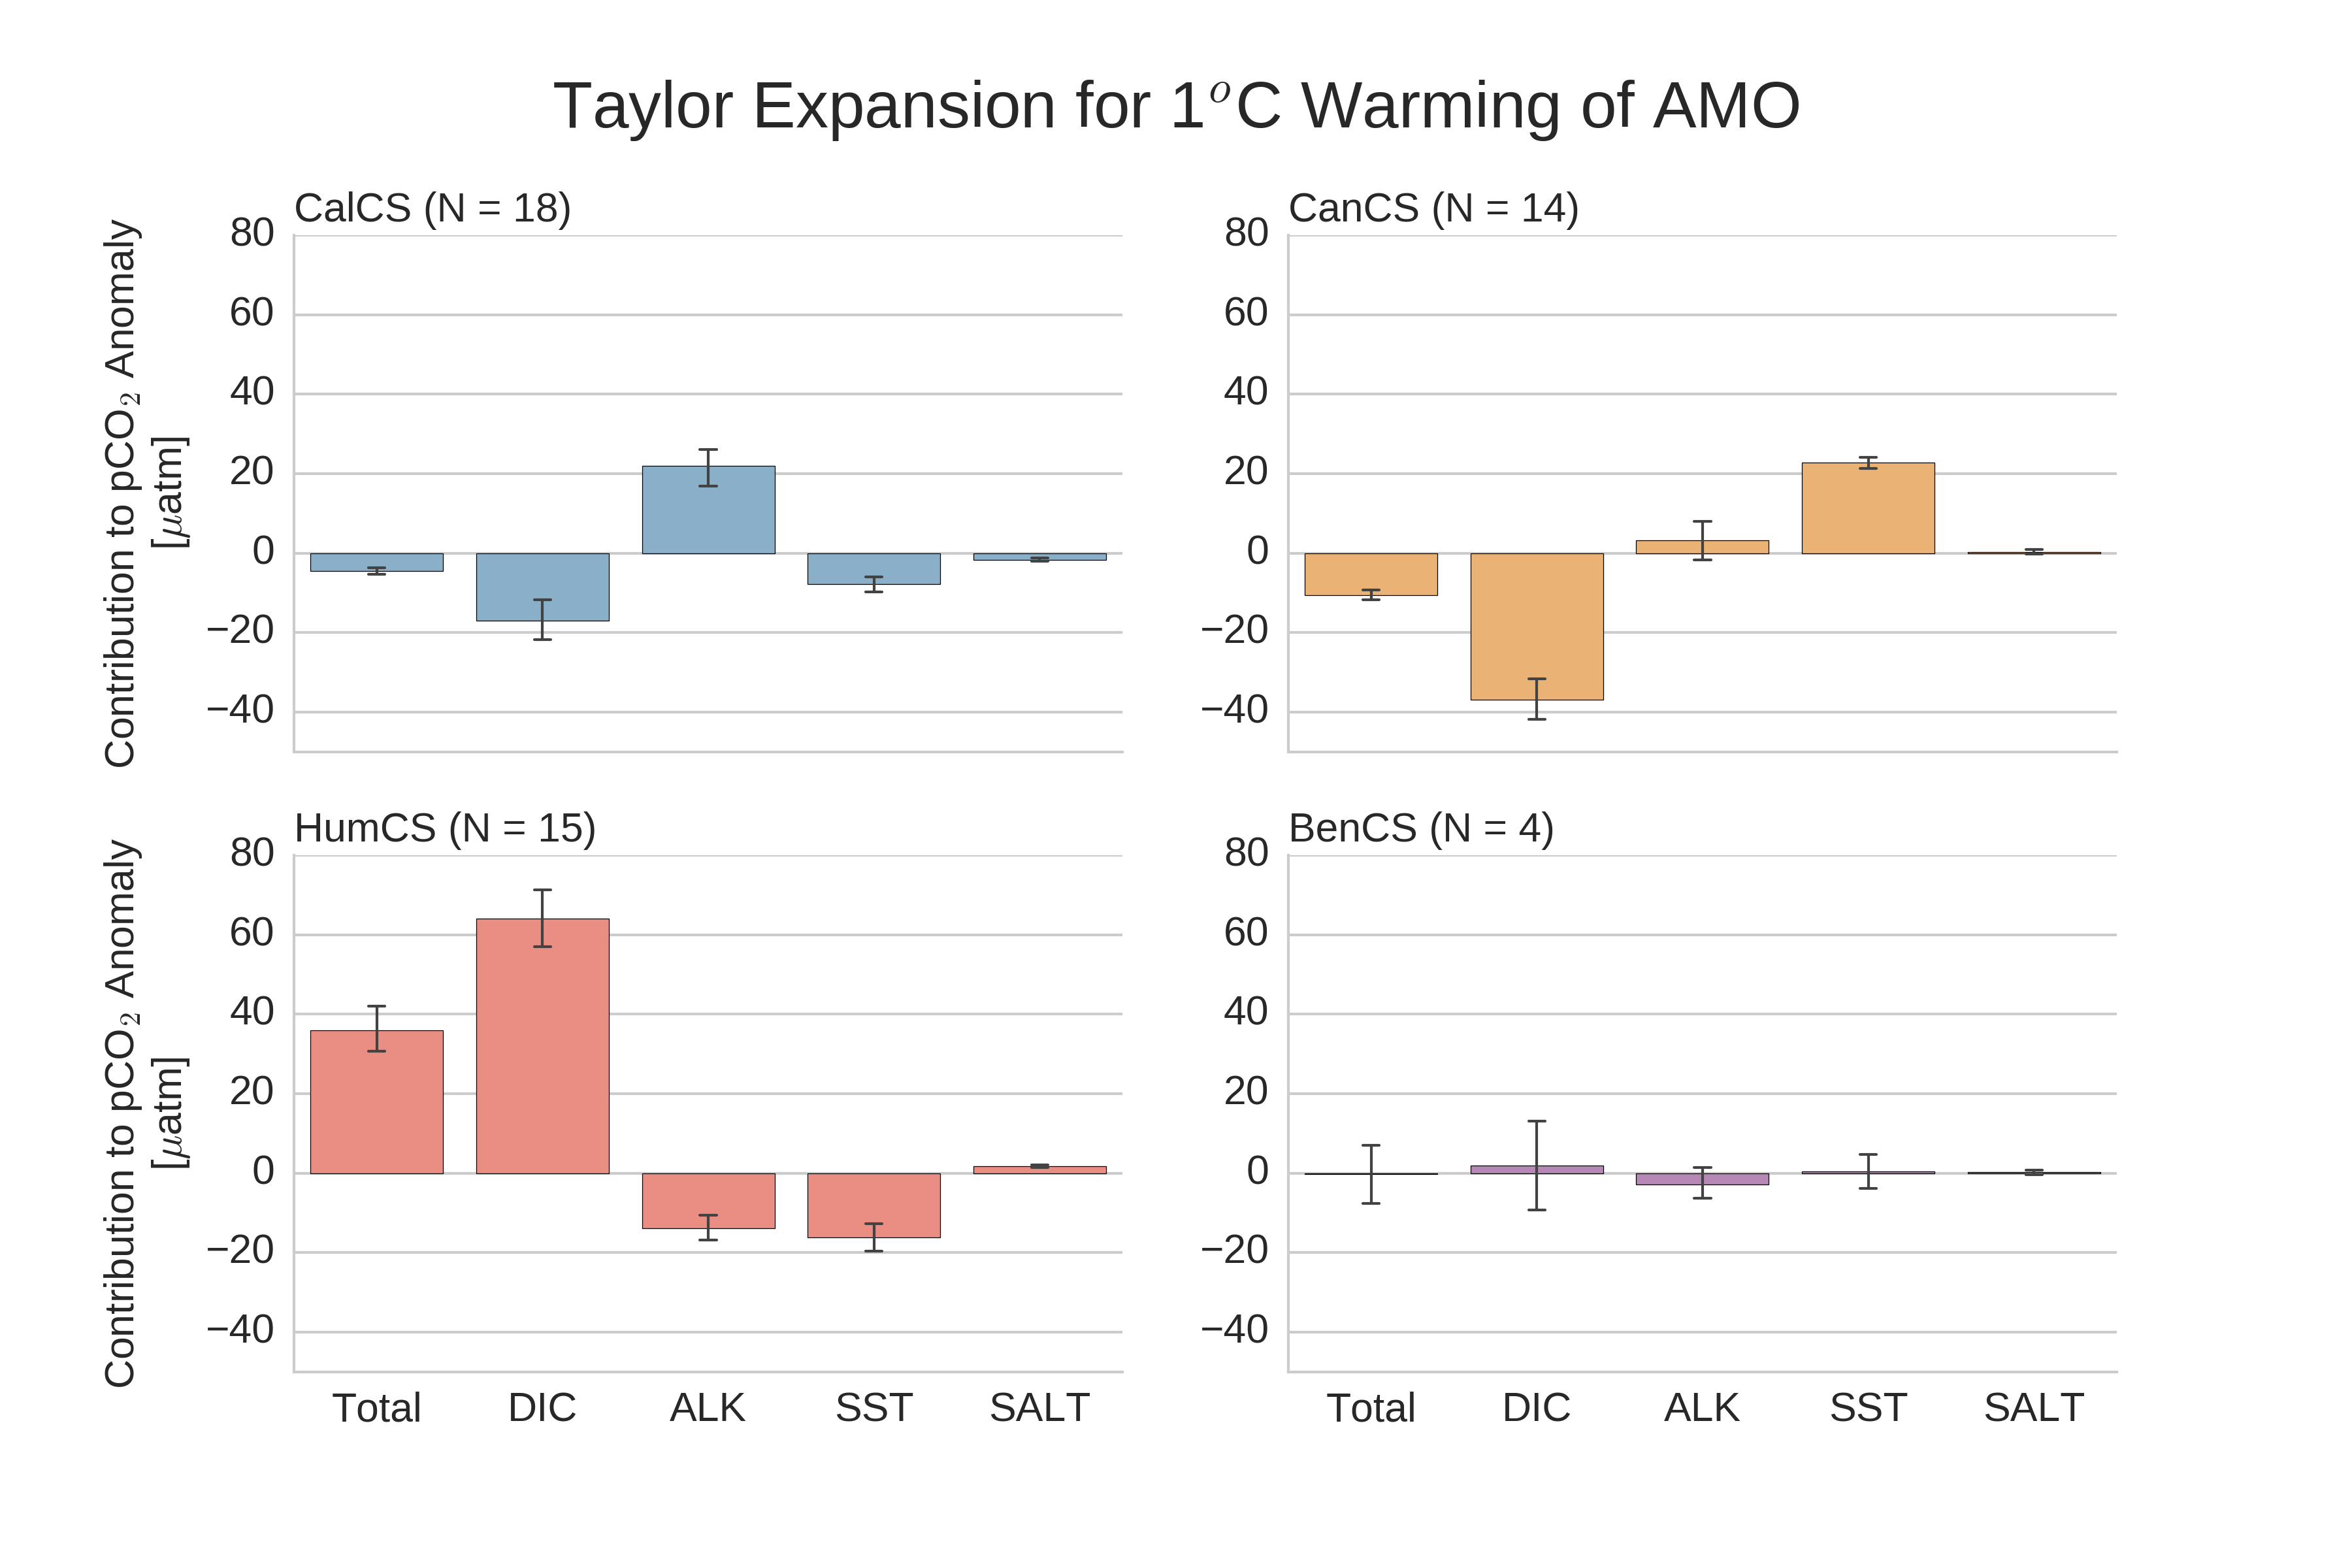
\includegraphics[width=\linewidth]{../../figs/all-systems/taylor_expansions/taylor-expansion-AMO-pCO2-PVALUEREMOVED-smoothedClimate.png}
	\caption{Linear Taylor Expansion of the relative contributions toward pCO$_{2}$ anomalies in a 1 degree C AMO event. Only simulations with $p$ $<$ 0.05 for pCO2, SALT, SST, ALK, and DIC were included.}
	\label{fig:taylor-amo}
\end{figure}
\begin{table}[!h]
	\centering
	\begin{tabular}{c | c c c c }
		& CalCS & HumCS & CanCS & BenCS \\
		\midrule
		Model Regression & -4.85 & 30.0 & -5.43 & 4.58 \\
		Taylor Summation & -4.48 & 36.0 & -10.51 & -0.25 \\
	\end{tabular}
	\caption{Comparison between regressing pCO$_{2}$ anomalies onto AMO and the summation of each term of the linear taylor approximation for each system}
	\label{tab:taylor-amo}
\end{table}

\clearpage
\begin{figure}[!h]
	\centering
	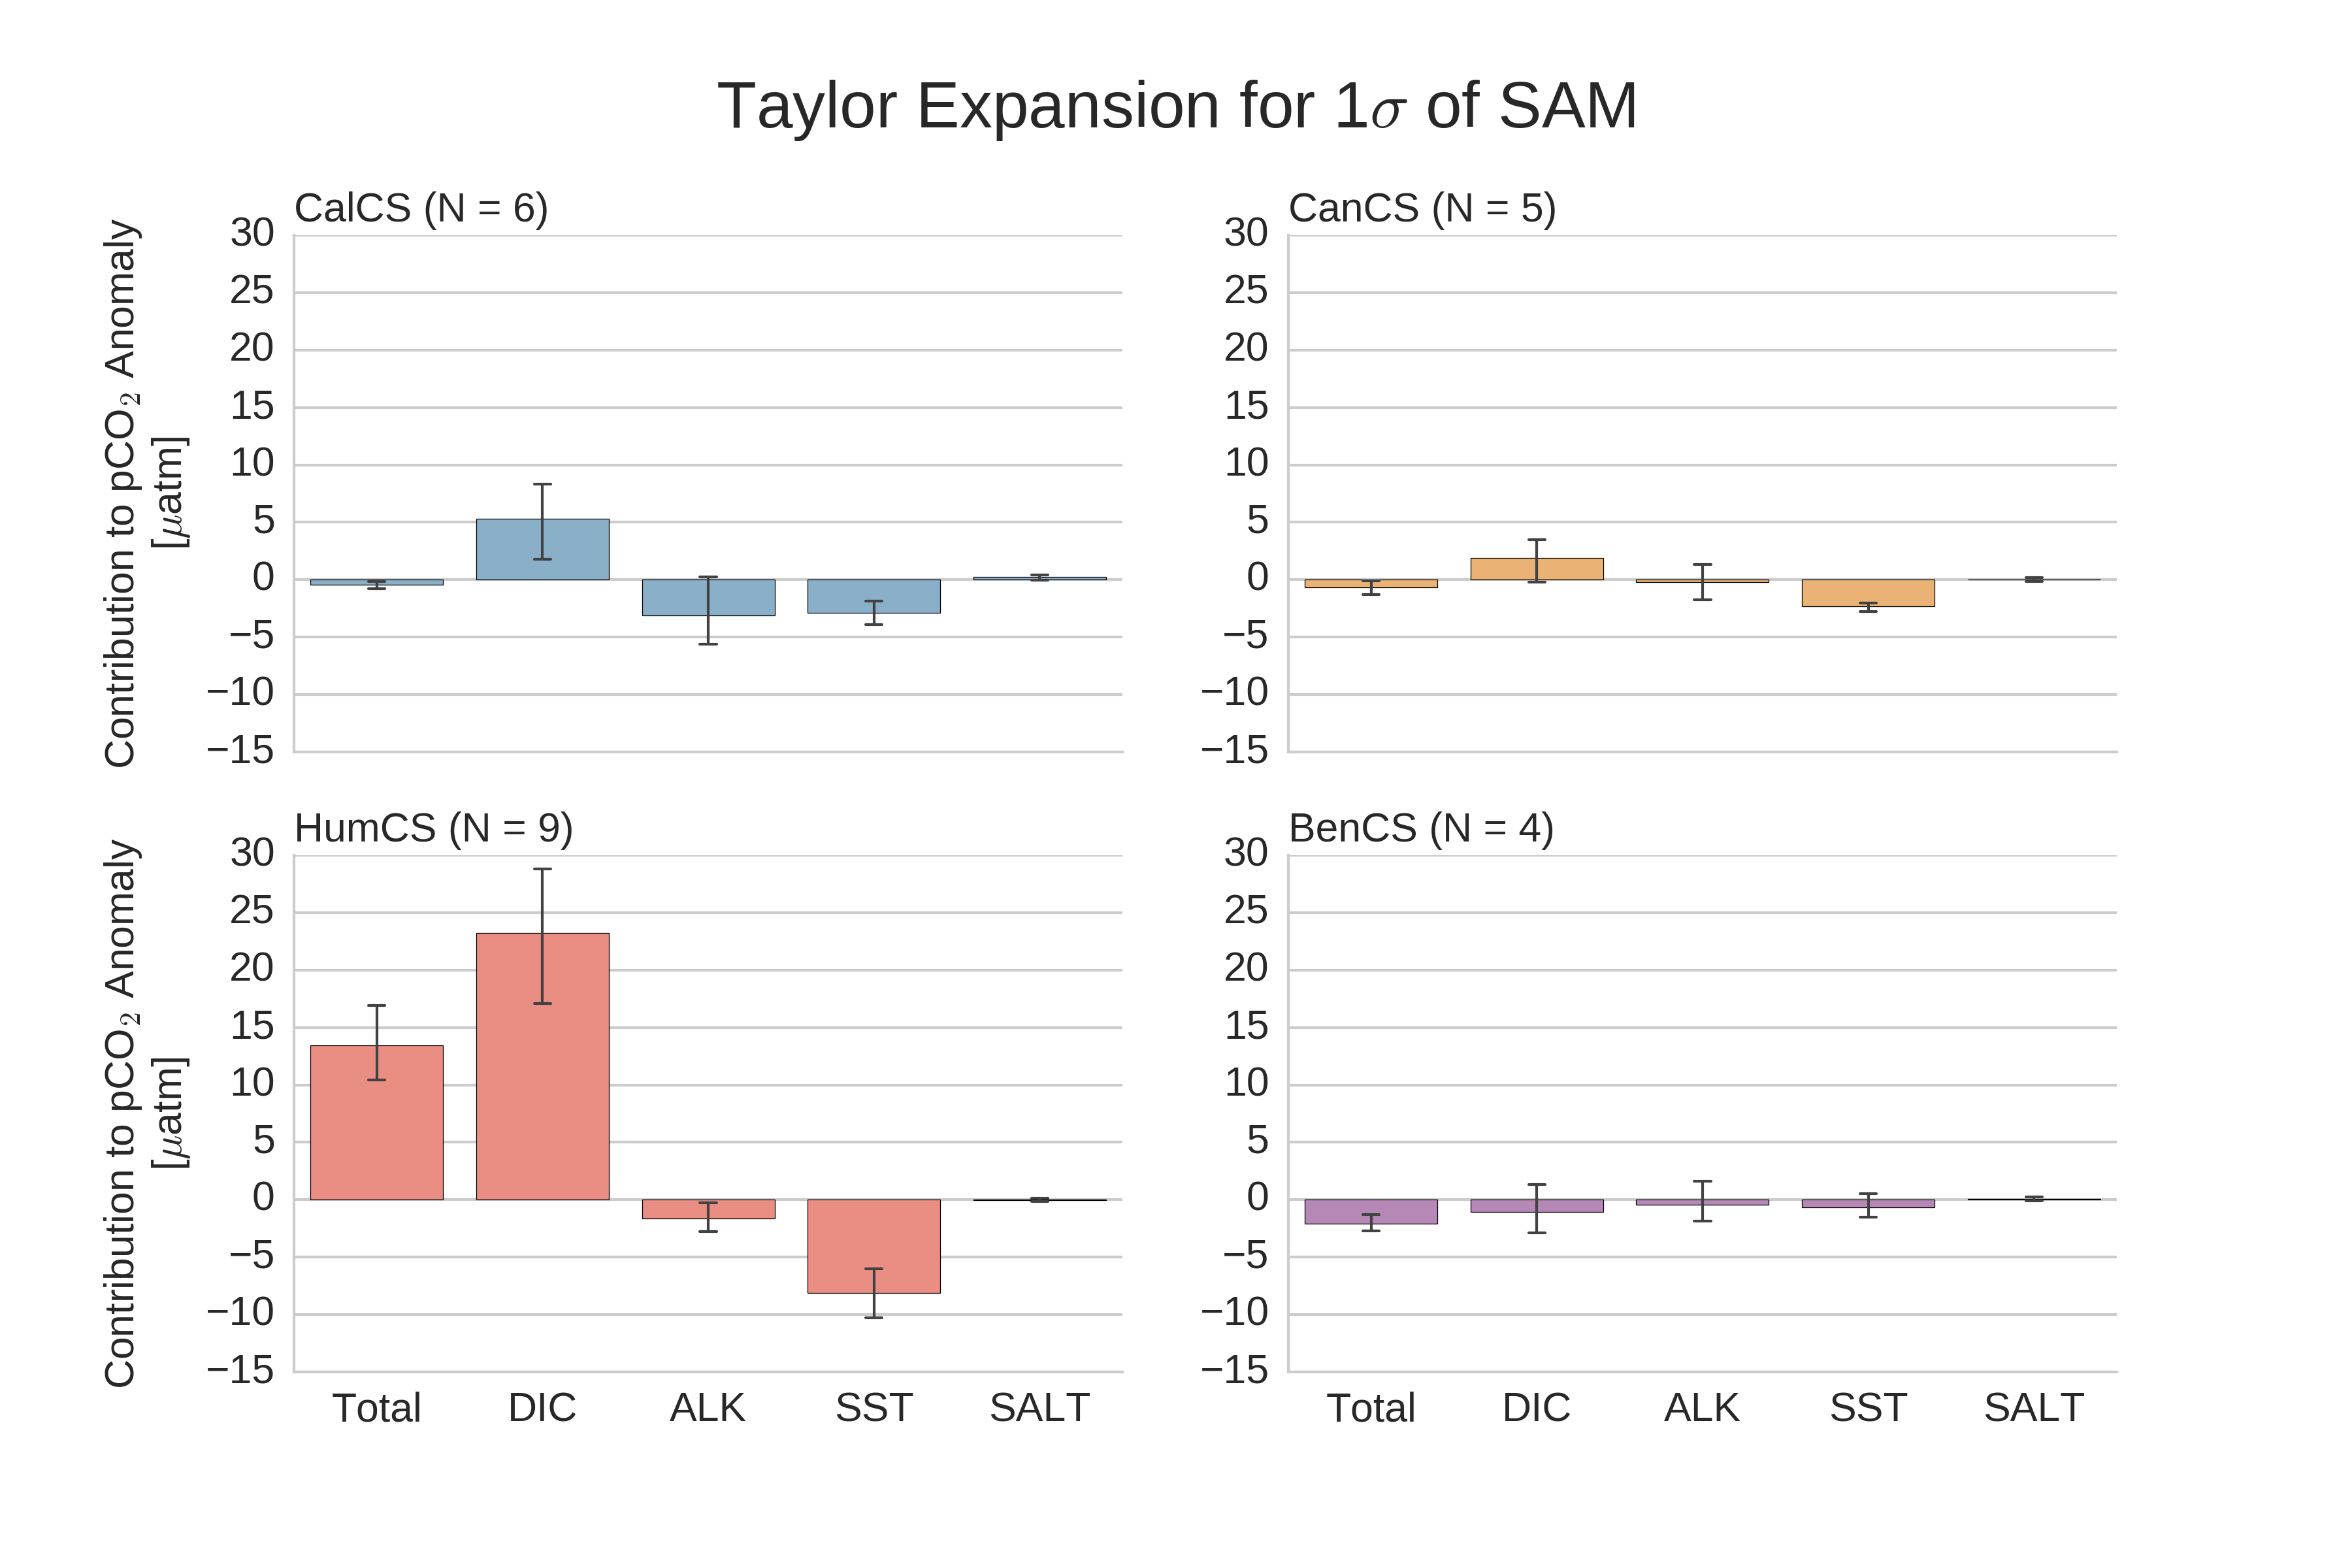
\includegraphics[width=\linewidth]{../../figs/all-systems/taylor_expansions/taylor-expansion-SAM-pCO2-PVALUEREMOVED-smoothedClimate.png}
	\caption{Linear Taylor Expansion of the relative contributions toward pCO$_{2}$ anomalies in a 1 $\sigma$ SAM event. Only simulations with $p$ $<$ 0.05 for pCO2, SALT, SST, ALK, and DIC were included.}
	\label{fig:taylor-sam}
\end{figure}
\begin{table}[!h]
	\centering
	\begin{tabular}{c | c c c c }
		& CalCS & HumCS & CanCS & BenCS \\
		\midrule
		Model Regression & -0.80 & 10.50 & -0.71 & -1.57 \\
		Taylor Summation & -0.46 & 13.44 & -0.67 & -2.08 \\
	\end{tabular}
	\caption{Comparison between regressing pCO$_{2}$ anomalies onto SAM and the summation of each term of the linear taylor approximation for each system}
	\label{tab:taylor-sam}
\end{table}

\clearpage
\bibliography{../../EBUS_BGC_Bibliography.bib}
\end{document}